\section{Experiments}
\label{sec:experiments}

We organize the evaluation around two questions: whether event-aligned spline actions improve execution from piecewise language, and whether their learned duration provides useful temporal control. Broad benchmark success provides context for both interventions.

\subsection{Setup}

\textbf{Policies and data.} All heads use the same 450M-parameter SmolVLA backbone \cite{shukor2025smolvla}. Waypoint A predicts 50 action tokens; fixed-window spline B uses eight control points and a 20-command target; event spline C uses eight control points and predicts duration. The broad LIBERO study trains each for 100,000 updates with batch size 32 on the same 40-task dataset, with three training seeds. The clause study begins from the corresponding 100,000-update A and C checkpoints, crossing whole-task and clause-aligned training labels. It uses 7,500 updates, batch size 32, and the same physical episodes for every treatment. Evaluation uses the final checkpoint rather than selecting the best checkpoint on test outcomes.

\textbf{Evaluation.} LIBERO \cite{liu2023libero} supplies four ten-task suites. The language experiment uses two multi-object LIBERO-Long tasks: soup and tomato into a basket (t0), and two mugs onto different plates (t4). Each condition evaluates the same 50 simulator states per task and three training seeds. The primary comparison sets $K=10$ and the same fixed clause schedule for both heads. Exact replays verify initial observations, simulator states, prompts, action traces, and outcomes. Replay repeats are checks, not additional independent trials.

RoboCasa365 \cite{nasiriany2026robocasa365} tests KettleBoiling and RinseSinkBasin on a targeted scene split, with official full-task success predicates. CALVIN \cite{mees2022calvin} uses the official list of five-instruction chains and reports mean consecutive tasks completed. The existing timing study evaluates 1,000 chains per checkpoint seed. Success percentages always refer to complete tasks unless a stage metric is named explicitly.

\textbf{Uncertainty.} For the primary language interaction, we report the effect for each of three trained policies and the $t$ interval over their training seeds. A hierarchical bootstrap resamples seeds and paired task/state outcomes as a sensitivity analysis. For binary paired interventions we use exact McNemar tests; the reported tests of RoboCasa phase labels use Fisher's exact test. CALVIN's historical intervals resample paired chains for the evaluated checkpoints; they are not population intervals over possible training runs.

\subsection{Question 1: Does the Action Head Affect Piecewise Language Execution?}

The language dataset contains 33 demonstrations of t0 and 38 of t4: 71 episodes and 19,378 frames. Table~\ref{tab:language} crosses the training labels with the inference interface. The scheduled columns use the same clauses and transition times regardless of training treatment. This holds the requested language program fixed while testing whether the policy learned to execute it.

\begin{table}[t]
\centering
\caption{LIBERO-Long t0/t4 success (\%). Each cell contains 300 rollouts: 50 states/task $\times$ two tasks $\times$ three training seeds. Columns change inference; rows change training labels.}
\label{tab:language}
\setlength{\tabcolsep}{5pt}
\begin{tabular}{llrr}
\toprule
 & & \multicolumn{2}{c}{Inference instruction} \\
\cmidrule(lr){3-4}
Head & Training labels & Static whole & Clauses \\
\midrule
Waypoint & Whole-task & 49.0 & 7.0 \\
Waypoint & Clauses & 39.7 & 41.3 \\
\addlinespace
Event spline & Whole-task & 57.0 & 11.7 \\
Event spline & Clauses & 33.0 & \textbf{55.3} \\
\bottomrule
\end{tabular}
\end{table}

\begin{figure*}[t]
\centering
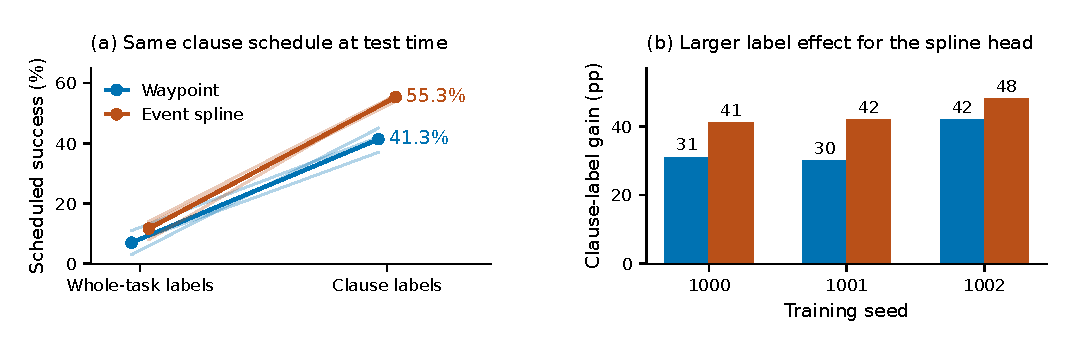
\includegraphics[width=\textwidth]{figures/language_v2.pdf}
\caption{Clause-aligned training improves execution under the same fixed clause schedule. (a) Absolute success on t0/t4; faint lines show individual training seeds and thick lines show their means. (b) The label effect for each seed. The difference between the spline and waypoint effects is +10, +12, and +6 percentage points.}
\label{fig:language}
\end{figure*}

Under scheduled clauses, success rises from 7.0\% to 41.3\% for the waypoint head and from 11.7\% to 55.3\% for the event spline. The label effects are +31, +30, and +42 points for A, and +41, +42, and +48 for C (Fig.~\ref{fig:language}). Define the head interaction at the fixed schedule as
\begin{equation}
 \Delta=(S_{C,\mathrm{clause}}-S_{C,\mathrm{whole}})
        -(S_{A,\mathrm{clause}}-S_{A,\mathrm{whole}}),
 \label{eq:interaction}
\end{equation}
where the second subscript denotes \emph{training labels}. Its mean is +9.33 points, with a 95\% $t$ interval of [1.74, 16.92] over training seeds and a hierarchical interval of [0.67, 18.0]. The advantage is therefore not limited to a single training run. It concerns the event spline head as a whole; this experiment does not separately identify the contributions of control-point count, event boundaries, and duration supervision.

The static columns provide an important control. Whole-caption-trained policies remain competent when given their native whole-caption input. Clause training does not improve this interface: it reduces static-prompt success by 9.3 points for A and 24.0 for C. The useful result is improved \emph{addressability through a clause program}, not a universal increase in canonical-task success. With the spline head, programmed success reaches 55.3\%, close descriptively to the whole-caption model's 57.0\%, while allowing the subgoal instruction to change during execution.

\textbf{Switching without a fixed demonstration clock.} Advancing the spline's clauses after its gripper opens yields 164/300 successes for clause training and 43/300 for whole-caption training: a 40.3-point label effect. This retains the direction and scale of the result obtained with a fixed clause schedule. It uses an action-derived switch, not the scalar duration prediction or an oracle goal predicate.

\subsection{Changing the Requested Subgoal Order}

We reverse the two clauses and score which official goal predicate becomes true first. This diagnostic uses a privileged predicate to advance to the second clause. On t4, both heads exhibit 10/50 paired states in which the first completed object changes in the requested direction, with no changes in the opposite direction (two-sided sign test $p=.00195$). Of 12 states with a unique first goal under both orders, 10 switch as requested.

\begin{table}[t]
\centering
\caption{Order intervention. First-object flips are measured on t4 (50 paired states); final task counts pool t0/t4 (100 states). All policies here are clause-trained.}
\label{tab:order}
\setlength{\tabcolsep}{4pt}
\begin{tabular}{lccrr}
\toprule
 & \multicolumn{2}{c}{First-object flips} & \multicolumn{2}{c}{Final success} \\
\cmidrule(lr){2-3}\cmidrule(lr){4-5}
Head & Requested & Opposite & Normal & Reverse \\
\midrule
Waypoint & 10/50 & 0/50 & 49/100 & 16/100 \\
Event spline & 10/50 & 0/50 & 55/100 & 21/100 \\
\bottomrule
\end{tabular}
\end{table}

The intervention changes behavior, but final conjunction success falls under reversed order (Table~\ref{tab:order}). The policy can respond to the first requested subgoal without reliably preserving it while completing the second. This separates first-subgoal steering from compositional generalization, and does not imply a spline-specific order advantage.

\subsection{Semantic Phases on RoboCasa365}

RoboCasa tests whether language alignment helps longer sequences involving grasping, transport, and fixture actuation. We use the same event-spline architecture and relabel identical demonstrations with official semantic phases. KettleBoiling has 501 demonstrations and 228,349 frames; RinseSinkBasin has 509 demonstrations and 211,036 frames. Within each seed, whole-caption and phase-label policies share initialization and receive 30,000 updates at batch size 32. Both are evaluated under the same outcome-independent phase schedule: Kettle switches at steps 128 and 242; Rinse switches at 162. These are demonstration-derived constants, not test-time success signals.

\begin{table}[t]
\centering
\caption{RoboCasa full-task success counts under the same fixed phase schedule. $n$ gives the number of trials per row and label treatment. Combined rows sum the two tasks.}
\label{tab:robocasa}
\setlength{\tabcolsep}{4.5pt}
\begin{tabular}{llrrr}
\toprule
Seed & Task & $n$ & Whole labels & Phase labels \\
\midrule
1000 & Kettle & 50 & 2 & 6 \\
 & Rinse & 50 & 2 & 10 \\
 & Combined & 100 & 4 & \textbf{16} \\
\addlinespace
1001 & Kettle & 20 & 2 & 1 \\
 & Rinse & 20 & 1 & 8 \\
 & Combined & 40 & 3 & \textbf{9} \\
\bottomrule
\end{tabular}
\end{table}

The two-task aggregate improves by 12 points on seed 1000 and 15 on seed 1001 (Table~\ref{tab:robocasa}). The first aggregate has Fisher $p=.00808$. Rinse improves on both seeds; Kettle's improvement does not replicate in the smaller evaluation of the second training seed. The result compares labels on two tasks in selected scenes; it is not an estimate over all 365 tasks or a waypoint--spline interaction on RoboCasa.

Stage measurements help locate the improvement. On seed 1000, phase labels increase Kettle grasp attainment from 24/50 to 39/50, and Rinse attainment of water-on with at least one washed region from 7/50 to 22/50. The latter improves from 3/20 to 12/20 on seed 1001. These intermediate counts are not substituted for full-task success.

The teaser follows one successful phase-trained Kettle rollout from a paired evaluation. Its whole-caption-trained counterpart begins from the identical observation and also grasps and reaches the stove. Only the phase-trained policy completes burner actuation: success at 516 steps versus failure at the 1,500-step limit. This paired example localizes the difference to the final stage.

\subsection{Question 2: What Does the Learned Physical Clock Enable?}

The timing experiments change the decoder of an already trained policy. CALVIN is a useful test because its human demonstrations include pauses and variable pace. The event head uses eight control points, $T_{\min}=8$, and $T_{\max}=16$ at the policy's 10-Hz action rate. Each command is held for three native simulator steps, preserving the replay-validated action convention. Every subtask receives the official 360-simulator-step budget.

\begin{figure*}[t]
\centering
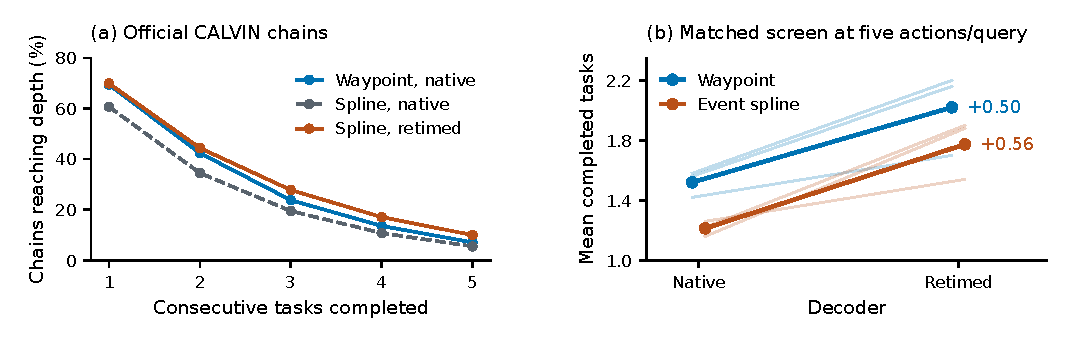
\includegraphics[width=\textwidth]{figures/clock_v3.pdf}
\caption{CALVIN timing results. (a) Historical study with 1,000 official chains per training seed. The waypoint comparator uses its native decoder. (b) Fresh screen with 50 common chains per seed and five actions per policy query. Thin lines show individual training seeds; thick lines show means. Both representations benefit from retiming.}
\label{fig:clock}
\end{figure*}

\begin{table}[t]
\centering
\caption{CALVIN mean consecutive tasks completed. Retiming uses $\alpha=0.6$, with actuator clipping and no feasibility stretch. Each seed has 1,000 chains.}
\label{tab:calvin}
\setlength{\tabcolsep}{4pt}
\begin{tabular}{lrrrr}
\toprule
Policy / decoder & 1000 & 1001 & 1002 & Mean \\
\midrule
Waypoint / native & 1.510 & 1.764 & 1.416 & 1.563 \\
Spline / native & 1.422 & 1.239 & 1.273 & 1.311 \\
Spline / retimed & 1.734 & 1.579 & 1.759 & \textbf{1.691} \\
\bottomrule
\end{tabular}
\end{table}

Uniform retiming improves the spline for every training seed (Table~\ref{tab:calvin}), with a mean gain of 0.379 completed tasks over paired chains (95\% CI [0.318, 0.441]). Realized pace is 1.42$\times$ the original spline, rather than the nominal $1/0.6=1.67\times$, because rounding, replanning, and changed behavior also affect completion time. The retimed spline exceeds the native waypoint by 0.127 tasks on average (95\% CI [0.063, 0.191] over paired chains), while first-task success is similar, 69.9\% versus 69.4\%. Figure~\ref{fig:clock} shows that the difference is concentrated in sustaining longer chains. This historical comparison uses a native waypoint decoder; the interpolation control below addresses that limitation directly.

\textbf{Separating interpolation from learned representation.} Native waypoint replay does not answer whether a spline is a better representation for retiming. We therefore specify a four-arm comparison: native and linearly retimed waypoints, and native and uniformly retimed event splines. Both retimed arms use $\alpha=0.6$, interpolation or decoding in raw command units, the same bounds, and no feasibility stretch. All four issue five actions per neural query, so even the shortest retimed spline segment fits the common cadence. They use the same official chains, noise seeds for every chain and subtask, controller rate, and time budgets. Tests of identity, normalization with a nonzero mean, and endpoints precede closed-loop evaluation.

The matched screen confirms that interpolation is a strong baseline (Fig.~\ref{fig:clock}b). Linear waypoint retiming raises mean chain length from 1.52 to 2.02; spline retiming raises it from 1.21 to 1.77. The corresponding gains are 0.50 and 0.56 tasks, giving an interaction of 0.06 (95\% $t$ interval over training seeds [$-0.87$, 0.99]). Thus temporal resampling itself is not unique to splines. The distinction is that the event spline predicts a duration that can decide \emph{which} segments to retime and \emph{when} to query again. The screen uses 50 official chains for each of three training seeds.

\textbf{Using duration as a control signal.} Retiming is only one use of the physical clock. Table~\ref{tab:clock_uses} collects three interventions that ask whether the predicted timing remains operational under changes to policy queries, language, and controller rate. These are targeted tests rather than additional headline tasks.

\begin{table*}[t]
\centering
\caption{Three uses of the learned physical clock. Policy weights remain fixed in every intervention.}
\label{tab:clock_uses}
\setlength{\tabcolsep}{10pt}
\begin{tabular}{lll}
\toprule
Control & Intervention & Outcome \\
\midrule
Query time & Replan at $\widehat T-4$ on LIBERO Object / Long & 2.68$\times$ / 2.24$\times$ fewer queries at matched success \\
Language pace & Add ``quickly'' on CALVIN & Commands +16\%; chain length 1.382 $\rightarrow$ 1.553 \\
Sampling rate & Execute at 2$\times$ on LIBERO Spatial t5 & Success 38$\rightarrow$68\% and 34$\rightarrow$72\% \\
\bottomrule
\end{tabular}
\end{table*}

The replanning result tests whether $\widehat T$ predicts a useful event time rather than merely serving as a decoder length. Replanning four actions before that time preserves the reference success on LIBERO Object and Long while using 2.68$\times$ and 2.24$\times$ fewer neural queries. The margin matters: waiting until $\widehat T$ reduces success to 84\% and 55\%, while margins of two and four actions improve monotonically. Duration can also select which motions to compress. On LIBERO Object, applying $\alpha=0.6$ only when $\widehat T>20$ yields 95\% success in 122.7 steps, compared with 93\% in 145.3 steps at the original pace and 73\% in 109.6 steps when every segment is compressed ($n=100$ each).

Language can also act on timing. We label CALVIN segments with kinematic adverbs derived from demonstration speed and train without changing their actions. At test time, ``quickly'' and ``slowly'' change issued pose-command magnitude by approximately +16\% and $-16\%$ relative to the same instruction without an adverb. The faster condition improves chain length from 1.382 to 1.553 over 600 chains ($p=.0175$, Bonferroni-corrected $p=.035$); the neutral prefix control gains only 0.025 tasks. This measures commanded motion and task completion, not guaranteed end-effector speed under arbitrary actuator limits.

Finally, changing the control rate while increasing the number of samples tests the distinction between duration and sampling density in Eq.~\ref{eq:decode}. On LIBERO Spatial t5, the event spline improves under twice the rate in two independently specified horizon protocols: 38\% to 68\% ($p=.00408$) and 34\% to 72\% ($p=.000311$), each on 50 paired states. The effect is task dependent: broad suite averages do not improve universally, so we use it as evidence that the curve can be resampled for controller adaptation rather than as a general success claim.

\subsection{General Task Performance}

Table~\ref{tab:libero} gives the four-suite context for these focused studies. Across three seeds, the event head averages 80.7\% against 82.1\% for waypoints, a 1.4-point difference at the native rate. The two-task language factorial is evaluated separately and is not folded into these suite averages.

\begin{table}[t]
\centering
\caption{Broad LIBERO success (\%). Three seeds, 1,200 rollouts/head across four suites. The final column is mean $\pm$ seed standard deviation of suite-averaged success.}
\label{tab:libero}
\setlength{\tabcolsep}{3pt}
\begin{tabular}{lrrrrr}
\toprule
Head & Object & Spatial & Goal & Long & Average \\
\midrule
Waypoint & 94.7 & 84.3 & 86.0 & 63.3 & $82.1\pm1.8$ \\
Fixed spline & 96.3 & 77.7 & 84.0 & 65.3 & $80.8\pm2.5$ \\
Event spline & 92.3 & 77.3 & 89.3 & 63.7 & $80.7\pm1.3$ \\
\bottomrule
\end{tabular}
\end{table}

\subsection{Real Robot Evaluation}
\label{sec:hardware}

\textit{Reserved for hardware results; no physical trials are claimed in this draft.} The planned setup uses one 7-DoF arm with a linear base, a gripper, and handheld teleoperation. The base remains fixed unless reach requires it. Existing printed fixtures support a short drawer program: open, insert an object, then close or leave open. The two final clauses share the same prefix, making the requested behavioral difference directly visible. A second feasible object-ordering task can test a changed sequence if demonstration collection permits.

The final section will report the collected demonstrations, train/test program split, matched policy comparisons, and complete-task counts on frozen initial configurations. A paired filmstrip that changes a late clause, together with a trajectory comparison before and after that change, will test whether the policy responds at the requested stage. The section will occupy approximately one page, including the result table and images. This is a focused test of language execution, not simply a deployment photograph.
